\documentclass[12pt]{book}
\usepackage{libertine}
\usepackage{libertinust1math}
\usepackage[T1]{fontenc}%coloca la ñ y acento
\usepackage[utf8]{inputenc} %coloca la ñ y acento 
\usepackage[spanish]{babel}
\usepackage{amsfonts,amstext,amssymb,amsthm}
\usepackage{graphicx}
\usepackage{enumerate}
\usepackage{style}
%%%%%%%%%%%%%%%%%%%%%%%%%%%%%%%%%%%%%
 
\begin{document}
%%%%%%%%%%%%%%%%%%%%%%%%%%%%%%%%%%%%
%%%%%%%%%%% INICIO DE CARATULA
\begin{titlepage}
\begin{center}
 \begin{figure}[htb]
\begin{center}

\includegraphics[width=8.5cm]{unmsm.jpg}
\vspace*{0.05in}
\end{center}
\end{figure}
%%%%%%%%
\rule{100mm}{0.1mm}\\
\vspace*{0.05in}
{\LARGE\textbf{FACULTAD DE CIENCIAS MATEMÁTICAS}}\\
\rule{100mm}{0.1mm}\\
\vspace*{0.20in}
{\large ESCUELA ACADÉMICO PROFESIONAL DE MATEMÁTICA}
\\
\textsf{\huge\textbf{  LA FUNCIÓN IMPLÍCITA}} \\
\vspace*{0.3in}
{\large Presentado por:}\\
\vspace*{0.3in}
{\Large Castro Tapia, Lejzer Javier\\Cumba Tinipuclla, Yuditd Araceli\\
Pino Espinoza, Renzo Anthony}
\vspace*{0.3in}\\
{\LARGE 2019}\\
\rule{80mm}{0.1mm}\\
\vspace*{0.1in}
\end{center}
\end{titlepage}
\tableofcontents
%%%%%%%%%%%%%%%%%%%%%%%%5
\chapter{Introducción al teorema de la función implícita}
\section{Funciones implícitas}
Cuando iniciamos como estudiantes de cálculo, usualmente una función es dada por una expresión analítica como:
$$f(x)=\sqrt{x^2+1}$$
$$h(t)=\cos(5t)$$
$$g(y)=y^3+6$$
De hecho, hace 250 años este fue el enfoque adoptado por Leonard Euler (1707-1783) cuando escribió: "Una función de una cantidad variable es una expresión analítica compuesta"
\\Casi inmediatamente, uno encuentra que la noción de "función dada por una fórmula" esta es demasiado limitado para los fines del cálculo.\\En contraste a la usual definición que se suele dar, una definición más precisa de \textit{función f con dominio X y rango Y} es la que sigue.
\begin{Def}
Una función con dominio X y rango Y es un subconjunto del producto cartesiano $X\times Y$ que cumple las siguientes propiedades:
\begin{enumerate}
    \item  Para cada $x\in X$ existe un elemento $(x,y)\in f$
    \item Si $(x,y)\in f$ y $(x,\tilde{y})\in f$, entonces $y=\tilde{y}$
\end{enumerate}
\end{Def} 
Por ejemplo, la siguiente expresión define un subconjunto de $\R^2$ descrita en la figura \ref{Figura1_1}\\
\begin{equation}
    y^5+16y-32x^3+32x=0
    \label{ecuacion1}
\end{equation}
\begin{figure}[htb]
\begin{center}
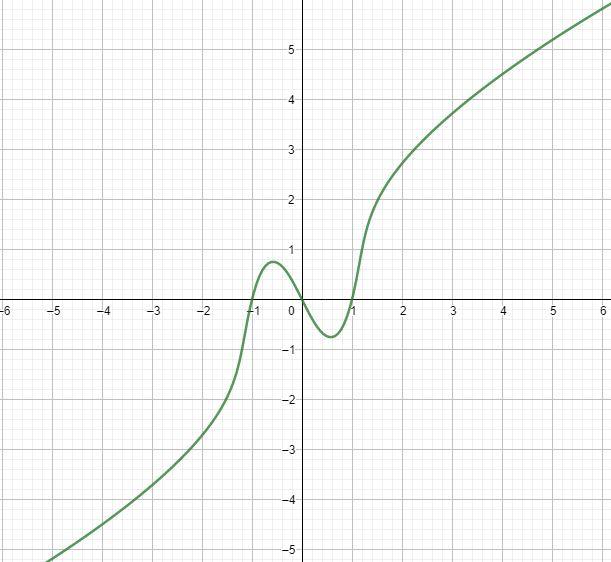
\includegraphics[width=8.5cm]{img/figura1_1.jpg}
\label{Figura1_1}
\caption{Gráfica de puntos que satisfacen \ref{ecuacion}}
\vspace*{0.05in}
\end{center}
\end{figure}
La gráfica nos muestra que aunque no se defina una fórmula explícitamente, con la definición previa el subconjunto $$f=\{(x,y)\in X\times Y: y^5+16y-32x^3+32x=0\}$$ es efectivamente una función. \\A este tipo de funciones las llamaremos \textit{funciones implícitas} y son ellas en las cuales nos centraremos en el desarrollo de este ensayo.
\chapter{La función implícita, un caso particular}
%parte de renzo%
\begin{Teo}
  $F:\mathbb{R}^2\rightarrow \mathbb{R}$ es de clase $C^{1}$, $(x_{0},z_{0}) \in \mathbb{R}^2$ tal que\\
  $F(x_{0},z_{0})=0$ y $ \frac{\partial F}{\partial Z}(x_{0},z_{0})\ne 0$\\
Entonces existen vecindades $U\ni x_{0} $ y $V\ni z_{0}$ y una funci\'on $C^1$:
    $$g:U\rightarrow V$$
   $$ \qquad \qquad x\longmapsto z=g(x)$$
Tal que $F(x,z)=0$ $\forall x \in U$, $\forall z\in V$ y :
$$\frac{\partial g}{\partial x} = - \frac{\frac{\partial F}{\partial x}}{\frac{\partial F}{\partial z}}$$
\end{Teo}
\begin{proof}
Supongamos que $\frac{\partial F}{\partial z}(x_{0},z_{0})>0$\\
\begin{Afi}
Existen $a,b > 0$ y $M>0$ tal que:\
\begin{center}
$ |x-x_{0}|<a$ y $|z-z_{0}|<a $ entonces  $\frac{\partial F}{\partial z}(x,z)>b$ y $|\frac{\partial F}{\partial x}(x,z)|\leq M$
\end{center}
\end{Afi}
En efecto :\
\begin{itemize}
    \item $\frac{\partial F}{\partial x}(x,z)$ es continua en $(x_{0},z_{0})$
\end{itemize}
Entonces $\forall \epsilon >0, \exists \delta >0$ tal que:\
   $$(x,z)\in \mathbb{R}^2 ||(x,z)-(x_{0},z_{0})||< \delta$$
    
    $ |\frac{\partial F}{\partial z}(x,z)-\frac{\partial F}{\partial z}(x_{0},z_{0})|< \epsilon$\\\\
    $\frac{\partial F}{\partial z}(x_{0},z_{0})- \epsilon < \frac{\partial F}{\partial z}(x,z) < \frac{\partial F}{\partial z}(x_{0},z_{0}) + \epsilon$
\begin{Obs}
$||(x,z)-(x_{0},z_{0})||< \delta $ $\Longleftrightarrow$ $|x-x_{0}|<\delta$ y $|z-z_{0}|<\delta$
\end{Obs} 
Se toma $$\epsilon=\frac{\partial F}{2\partial z}(x_{0},z_{0})>0$$ entonces 
    $\exists \delta > 0$ y $\exists b=\frac{\partial F}{2\partial z}(x_{0},z_{0})>0$ 
Tal que
    $\frac{\partial F}{\partial z}(x,z) > b$ si $|x-x_{0}|< \delta $ y $|z-z_{0}|< \delta$
\begin{itemize}
    \item $\frac{\partial F}{\partial z}(x,z)$ es continua en $(x_{0},z_{0})$
\end{itemize}
Entonces $\forall \epsilon >0, \exists \delta >0$ tal que
    $(x,z)\in \mathbb{R}^2$, $||(x,z)-(x_{0},z_{0})||< \delta'$\\
    
    $ |\frac{\partial F}{\partial x}(x,z)-\frac{\partial F}{\partial x}(x_{0},z_{0})|< \epsilon$ \\
    
    $ |\frac{\partial F}{\partial x}(x,z)|< (|\frac{\partial F}{\partial x}(x_{0},z_{0})|+\epsilon)$\\\\
Se toma $a \equiv min ({\delta ,\delta'})> 0$

\begin{Afi}
La funci\'on $F(x,z)$ se puede escribir en la forma siguiente: \\
\begin{eqnarray}
    F(x,z)= \frac{\partial F}{\partial x}(\theta x +(1-\theta)x_{0},z).(x-x_{0})+\frac{\partial F}{\partial z}(x_{0},\phi z +(1-\phi)z_{0}).(z-z_{0})
    \label{asterisco}
\end{eqnarray}
   \textit{Donde }$0< \theta$, $\phi <1$
\end{Afi}
En efecto :
%\begin{center}
    \begin{eqnarray}
   F(x,z)= F(x,z)-F(x_{0},z) = [F(x,z)-F(x_{0},z)] +  [F(x_{0},z)-F(x_{0},z_{0})]
   \label{uno}
    \end{eqnarray}
     \begin{itemize}
         \item $h(t)\equiv F(tx+(1-t)x_{0},z)$ (con x, y, z fijos)
     \end{itemize}
Entonces, por el el teorema del valor medio existe un número $\theta$ entre $0$ y $1$ tal que:\\
$$h(1)-h(0)=h'(\theta (1-0))$$\\Entonces: 
$$F(x,z)-F(x_{0},z)=\frac{\partial F}{\partial x}(\theta x + (1-\theta)x_{0},z)(x-x_{0}) $$
\begin{itemize}
    \item An\'alogamente :\ $J(t)\equiv F(x_{0},tz+(1-t)z_{0})$ (con z fijo)
\end{itemize}
Entonces, por el teorema del valor medio
\begin{eqnarray}
  |F(x_{0},z)-F(x_{0},z_{0})=\frac{\partial F}{\partial z}(x_{0},\phi z + (1-\phi)z_{0})(z-z_{0}) 
 \label{tres}
\end{eqnarray}
Donde $ \phi\in[0,1]$
\begin{Afi}
Existen $a_{0}, \delta > 0$ con $a_{0} < a$ y $\delta <a_{0}$ tal que:\\
$|x-x_{0}|<\delta$  entonces $F(x, z_{0}+ a_{0}) > 0$ y $F(x, z_{0}-a_{0}) < 0$
\end{Afi}
En efecto
\begin{itemize}
    \item Como $0<a_{0}$ y $\bar{\mathbb{Q}}= \mathbb{R}$, entonces $\exists a_{0}$ tal que $0< a_{0}<a $
\end{itemize}
\begin{itemize}
    \item $0 < a_{0}$ y $\bar{\mathbb{Q}}= \mathbb{R}$, entonces $\exists \delta_{1}$ tal que $0 < \delta_{1} < a_{0}$\\
    
    $0 < \frac{ba_{0}}{M} $, entonces $\exists \delta_{2}$ tal que $0 < \delta_{2} < \frac{ba_{0}}{M}$\\
    
    Tomo $\delta = min(\delta_{1},\delta_{2}) > 0$, entonces $\exists \delta > 0$ tal que $\delta < a_{0}, \frac{ba_{0}}{M}$
\end{itemize}

\begin{itemize}
    \item Si $|x-x_{0}| < \delta$\\\\
    Entonces $|x-x_{0}| < a $\\
    En consecuencia \\\\
    $\left(
      \begin{matrix} 
         |\frac{\partial F}{\partial x}(\theta x + (1-\theta)x_{0}, z)(x-x_{0})| \\\\
         = |\frac{\partial F}{\partial x}(\theta x + (1-\theta)x_{0}, z)||(x-x_{0})|
      \end{matrix}
   \right \}$\\\\ \\$|\theta x + (1-\theta)x_{0}-x_{0}|= |\theta x - \theta x_{0}|= |\theta||x-x_{0}|\leq|x-x_{0}|< a_{0}<a$ $< M\delta <M\frac{ba_{0}}{M}= ba_{0}$\\
Asi: $$|\frac{\partial F}{\partial x}(\theta x + (1-\theta)x_{0},z)(x-x_{0})|< ba_{0}$$\\
Si $|x-x_{0}|< \delta$, donde $z-z_{0}< a$
\end{itemize}
\begin{itemize}
    \item En \ref{asterisco}, se toma $z=z_{0}+a_{0}$,\
    $F(x,z_{0}+a_{0})= \frac{\partial F}{\partial x}(\theta x + (1-\theta)x_{0},z_{0}+a_{0}).(x-x_{0})+ \frac{\partial F}{\partial z}(x_{0},\phi a_{0}+z_{0}).a_{0} > -ba_{0} + ba_{0}> 0$
\end{itemize}
\begin{itemize}
    \item An\'alogamente $F(x,z_{0}-a_{0})< 0 $
\end{itemize}
Sean $U$ la vecindad de centro $x_{0}$ y radio $\delta$, $V$ la vecindad de centro $z_{0}$ y radio $a_{0}$\\
Fijemos $x\in U$, y definamos la funci\'on:
\begin{center}
    $k:V \rightarrow \mathbb{R}$\\
    $\qquad \qquad \qquad \qquad z\longrightarrow k(z)\subseteq F(x,z)$
\end{center}
Se sigue que $K\in C^{1}$, y como $K(z_{0}+a_{0})>0$ y $K(z_{0}-a_{0})<0 $\\
Por el TVI: $\exists z\in V$ tal que $K(a)=0$\\
Entonces: $F(x,z)=0$ y como $K'=\frac{\partial F}{\partial z} > 0$, $z \in \delta$ \textit{tal que } $$\forall x\in \exists!z\in V \textit{tal que} F(x,z)=0$$
Esto permite definir la funci\'on :
\begin{center}
    $g:U \rightarrow V$\\
    $\qquad \qquad  x\longrightarrow z=g(x)$
\end{center}
de tal forma que $F(x,z)=0$, $\forall x\in U$, $\forall z\in V$\\
\begin{Afi}
 $g: U \rightarrow V $es continua\\
 \end{Afi}
 En efecto: Sea $x_{0}\in U$, por demostrar: \\
 \begin{center}
     $g$ es constante  en $x_{1}$ $\Longleftrightarrow\lim_{x \to x_{0}}g(x)=g(x_{0})$\\ $$\Longleftrightarrow \lim_{x \to x_{0}}g(x)-g(x_{0})=0 \Longleftrightarrow\lim_{x \to x_{0}}z-z_{0}=0$$
 \end{center}
 De \ref{asterisco}\\
      $$z-z_{0}=-\frac{\frac{\partial F}{\partial x}(\theta x+(1-\theta)x_{0},z)(x-x_{0})}{\frac{\partial F}{\partial z }(x_{0}, \phi z + (1-\phi)z_{0})}$$
 Entonces:
    $$\lim_{x \to x_{0}}(z-z_{0})= -\frac{\frac{\partial F}{\partial x}(x_{0},z).0}{\frac{\partial F}{\partial z }(x_{0}, \phi z + (1-\phi)z_{0})}=0$$
\begin{Afi}
$g: U \rightarrow V $ es $C^{1}$
\end{Afi}
En efecto: 
\\Sea $x_0\in U$\\
   $$ \frac{g(x_{0}+h)-g(x_{0})}{h}=-\frac{\frac{\partial F}{\partial x}(\theta h+x_{0},z)}{\frac{\partial F}{\partial z }(x_{0}, \phi z+(1-\phi)z_{0} )}$$
   $$=-\frac{\frac{\partial F}{\partial x}(\theta h+x_{0},g(x_{0}+h))}{\frac{\partial F}{\partial z }(x_{0}, \phi g(x_{0}+h)+(1-\phi)g(x_{0}) )}$$
 $$g'(x_{0})=\lim_{h \to 0}\frac{g(x_{0}+h)-g(x_{0})}{h} =-\frac{\frac{\partial F}{\partial x}(x_{0},g(x_{0}))}{\frac{\partial F}{\partial z }(x_{0}, g(x_{0})) )}\in C^{1}$$
$$\therefore g \in C^{1}$$
\end{proof}
\chapter{El teorema de la función implícita, caso general}

Para llegar al objetivo de demostrar el teorema de la función implícita, se usará principalmente el teorema de la función inversa y el teorema de la forma local de las sumersiones. Las demostraciones de estos teoremas se encontrarán citadas para el lector interesado.
\section{Preliminares}
Se debe tener en cuenta que los puntos del espacio $\R^{m+n}$ serán representados de la forma $p=(a,b)$, donde $a\in\R^m$ y $b\in\R^n$.
\begin{Teo}(Teorema de la función inversa)\\
Sea $U\subseteq\R^m $ abierto, $f\in C^k(U,\R^m), k\in\N$ tal que $f'(a)\in GL(\R^m)$ (donde $a\in U$). Entonces existen vecindades $W\subseteq U$ y $V\subseteq\R^m$ de a y f(a) respectivamente tal que $f:W\rightarrow V$ es un difeomorfismo de clase $C^k$.\\
(\textnormal{Ver demostración en} Lages \cite{lagesflaco} [pág. 115-116])
\end{Teo}
\begin{Def}
Sea $U\subseteq\R^m $ abierto, $f:U\rightarrow\R^m$ una función diferenciable en U. Se dice que f es una sumersión de U en $\R^n$ si y solo si $f'(x)\in\mathcal{L}(\R^m,\R^n)$ es sobreyectiva.
\end{Def}
El teorema siguiente nos muestra que una sumersión puede comportarse localmente como una proyección. Su demostración usa el teorema de la función inversa.
\begin{Teo}(Formas locales de las sumersiones)\\
\label{sumersiones}
Sea $U\subseteq\R^{m+n} $ abierto, $f\in C^k(U,\R^n), k\in\N$. Sea $p=(a,b)\in U$ donde $a\in\R^m$ y $b\in\R^n$. Si $f'(p)\in GL(\R^m)$ es sobreyectiva, entonces  existen vecindades $V\subseteq \R^m$, $W\subseteq\R^{n}$ y $Z\subseteq U$  de a, f(p) y p  respectivamente, tal que existe $h_p:V\times W\rightarrow Z$ tales que
\begin{enumerate}
    \item $h_p(a,f(p))=p$
    \item $(f\circ h_p)(v,w)=w$ \textbf{           } $\forall v\in V, w\in W$
\end{enumerate}
(\textnormal{Ver demostración en} Lages \cite{lagesflaco} [pág. 117-119])
\end{Teo}
\section{Teorema de las funciones implícitas}
Este teorema establece condiciones suficientes, bajo el conjunto de ecuaciones de varias variables permite definir a varias de ellas como función de las demás.
Es decir, localmente existe una función $y=f(x)$ que sustituida en la ecuación $F(x,y)=c$ , la convierte en una identidad matemática.
\begin{Teo}
Sea $U\subseteq\R^{m+n} $ abierto, $F=(F_1,\ldots,F_n):U\rightarrow\R^n$ de clase $C^k$. Supongamos que en un punto $p=(a,b)$ con $F(p)=c$ y la matriz $$\bigg[\frac{\partial F_i}{\partial y_j}(p)\bigg]\in GL(\R^n)\textsf{       i,j=1,\ldots,n}$$
Entonces existen vecindades $V\subseteq \R^m$, y $Z\subseteq U$  de a y p  respectivamente, y una función $f:V\rightarrow\R^n$ de clase $C^k$ tal que $b=f(a)$ y $$F(x,f(x))=c\textsf{,    }\forall x\in V$$
\end{Teo}
\begin{proof}
  \textsf{}\\Sea V, W, Z y h como en el teorema \ref{sumersiones}.\\Definamos $f:V\rightarrow    \R^n$ como $f(x)=h_2(x,c)$, donde $h_2:V\times W\rightarrow\R^n$ es la proyección a la segunda coordenada de h, es decir $h(x,w)=(x,h_2(x,w))$. Asimismo $(x,y)\in Z$ entonces $x\in V$ y $(x,y)=h(x,w),$ $w\in W$.\\si además se tiene f(x,y)=c, entonces c=f(x,y)=f(x,f(x)) e $y=(x)$.\\
Resumiendo: $(x,y)\in Z$ e $f(x,y)=c$ implican que $x\in V$ e $y=f(x)$.\\ Recíprocamente si $x\in V$ e $y=h(x)$ entonces $y=h_2(x,c)$ e $f(x,y)=f(x,h_2(x,c))=f(h(x,c))=c$
\end{proof}
\chapter{Aplicación a la geometría diferencial}
\section{Primeras definiciones y ejemplos}
Intuitivamente una curva en $\R^{3}$ es un conjunto que se puede identificar con un subconjunto de $\R$ (esto es, puede ser parametrizado por una función en una variable) y una superficie en $\R^{3}$ es un conjunto que se puede identificar con un subconjunto de $\R^{2}$  (esto es, puede ser parametrizado por una función en dos variables). El propósito de esta sección es formalizar estas nociones, extendiéndolas a la totalidad de espacios euclidianos y generalizándolas a términos locales, de manera que podamos clasificarlas por dimensión y regularidad.

\begin{Def}
Sea $V\subseteq\R^{n}$ y $k\in\N\cup\{\infty\}$, una parametrización de clase $C^{k}$ y dimensión $m$ del conjunto $V$ es un par $(U,\varphi)$, donde $U\subseteq\R^{m}$ es un abierto y $\varphi:U\rightarrow V$ es un homeomorfismo de clase $C^{k}$ con $\varphi'(x)\in L(R^{m},R^{n})$ inyectiva para todo $x\in U$.
\end{Def}

\begin{Obs}
En la definición, fijado $x_{0}\in U$, como $\varphi'(x_{0}):\R^{m}\rightarrow\R^{n}$ es una transformación lineal inyectiva, entonces $dim[\varphi'(x_{0})(R^{m})]=m\leq n$ (i.e. la dimensión de la parametrización no supera la dimensión del espacio hábitat del conjunto parametrizado.)
\end{Obs}

\begin{Obs}
En la definición, sea $\varphi=(\varphi_{1},...,\varphi_{n})$, para todo $p\in V$ existe $(x_{1},...,x_{m})=\varphi^{-1}(p)$ y tenemos que $p=(\varphi_{1}(x_{1},...,x_{m}),...,\varphi_{n}(x_{1},...,x_{m}))$ (i.e. todo $p\in V$ depende solo de $m$ coordenadas).
\end{Obs}
\begin{Def} Una superficie de dimensión $m$ y clase $C^{k}$ es un subconjunto $M\in\R^{n}$ tal que para todo punto $p\in M$ existe una vecindad abierta $U_{p}\in \R^{n}$ de $p$ tal que el conjunto $U_{p}\cup M$ admite una parametrización de clase $C^{k}$ y dimensión $M$.
\end{Def}

\begin{Obs}
$U_{p}\cup M$ es llamada \textit{vecindad parametrizada del punto $p$}.
\end{Obs}

\begin{Obs}
Las superficies de dimensión 1 son llamadas \textit{curvas} y las superficies de dimensión $n-1$ en $\R^{n}$ son llamadas \textit{hiperficies}.
\end{Obs}

\begin{Ejm}
Sea $V=S^{1}-\{0\}$, $V_{0}=]0,2\pi[$ ,
\begin{center}
    $\phi:V_{0}\rightarrow V$\\
    $\qquad \qquad \qquad  t\longrightarrow(\cos(t),\sin(t))$
\end{center} forman una parametrización de clase $C^{\infty}$ y dimensión 1 que funciona para todo punto $p\in V$, entonces V es una superficie de dimensión 1 (curva) y clase $C^{\infty}$. Este tipo de curvas se denominan simples.
\end{Ejm}

\section{Superficies definidas implícitamente}

\begin{Def}
Sea $U\in\R^{m}$ un abierto y $f:U\rightarrow\R^{n}$ una función diferenciable, decimos que $c\in\R^{n}$ es un valor regular de $f$ si y solo si $f'(x)\in L(\R^{m},\R^{n}$ es sobreyectiva para todo $x\in f^{-1}(c)$.
\end{Def}

\begin{Lem}
Si $U\in\R^{m}$ es un abierto y $f:U\rightarrow\R^{n}$ una función de clase $C^{k}$, entonces el gráfico de $f$, $G(f)=\{(x,f(x))\in \R^{m+n}:x\in U\}$, es una superficie de dimensión m y de clase $C^{k}$ de $\R^{m+n}$.
\end{Lem}

\begin{proof}
 Basta considerar el par $(U,\phi)$ donde $\phi:U\rightarrow G(f)$ está definida por $\phi(x)=(x,f(x))$, claramente $\phi$ es un homeomorfismo y su matriz $J(\phi(x))$ tiene rango $m$ para todo $x\in U$, esto es, $\phi'(x)$ es inyectiva para todo $x\in U$, luego, $(U,\phi)$ es una parametrización de clase $C^{k}$ y dimensión $m$ que funciona para todo punto $p\in G(f)$, por lo tanto, $G(f)$ es una superficie de dimensión $m$ y clase $C^{k}$ de $\R^{m+n}$.
\end{proof}

\begin{Teo}
Sea $U\in\R^{m}$ un abierto, $f\in C^{k}(U,\R^{n})$ y $c\in R^{n}$ un valor regular de $f$, entonces, $f^{-1}(c)\subseteq\R^{m}$ es una superficie de dimensión $m-n$ y de clase $C^{k}$.
\end{Teo}

\begin{proof}
Sea $p=(p',p'')\in f^{-1}(c)$, desde que $f'(p)\in L(\R^{m},\R^{n})$ es sobreyectiva, por el teorema de la función implícita, existen abiertos $Z_{p}\subseteq U$, $V_{p}\subseteq\R^{m-n}$ con $p\in Z_{p}$, $p'\in V_{p}$ y existe una función $\xi_{p}:V_{p}\rightarrow\R^{n}$ de clase $C^{k}$ tal que $G(\xi_{p})=\{(x,\xi_{p}(x)):x\in V_{p}\}=Z_{p}\cup f^{-1}(c)$.\\Sea $\phi_{p}:V_{p}\rightarrow Z_{p}\cup f^{-1}(c)$ definida por $\phi_{p}(x)=(x,\xi_{p}(x))$, luego, por el lema anterior, $(V_{p},\phi_{p})$ es una parametrización de clase $C^{k}$ y dimensión $m-n$ de $Z_{p}\cup f^{-1}(c)$, así, $f^{-1}(c)$ es un superficie de dimensión $m-n$ y clase $C^{k}$.
\end{proof}

\begin{Obs}
En el siguiente ejemplo mostraremos uno de los potentes usos del teorema anterior. 
\end{Obs}

\begin{Ejm}(La esfera $S^n$ definida implícitamente)
\begin{center}
    $f:\R^n \rightarrow \R$\\
    $\qquad \qquad  x\longrightarrow f(x)=\|x\|^2$
\end{center}
Se sigue que $\triangledown f(x)=2x$ y por 1 es valor regular es valor regular de f.\\ Como $f^{-1}=S^{n-1}$, se sigue que $S^{n-1}$ es una superficie de clase $C^\infty$ y codimensión 1. Más aún $$T_pS^{n-1}=Nu(f'(p))=\{h\in\R^n :\langle p,h \rangle=0\}=\langle p\rangle^\bot$$
\end{Ejm}
\begin{thebibliography}{}
\bibitem{lagesflaco}Lages E.(2004). \emph{Análise Real ,Volume 2}. Río de Janeiro, Brasil: Associação Instituto Nacional de Matemática Pura e Áplicada-IMPA

\bibitem{} Krantz, Steven G., Parks, Harold R. (2013). \emph{The Implicit Function Theorem}. Springer Science+Business Media New York.

\end{thebibliography}
\end{document}